\documentclass[12pt,usletter,english]{article}
\usepackage[utf8]{inputenc}
\usepackage{graphicx}
\usepackage{amsmath}
\usepackage{amssymb}
\usepackage{subcaption}
\usepackage[font={small}]{caption}
\usepackage{fancyhdr}
\usepackage{float}
\usepackage{listings}

\pagestyle{fancy}
\lhead{Problem Set 2} \rhead{Deepthi Gorthi}

\begin{document}
\title{PS2: Introduction to Probablity and Statistics} \author{Deepthi
  Gorthi\\ AY250: Stellar Populations} \maketitle

\section{Problem 1}

There is a minor mistake on the Initial Mass Function page of
Wikipedia.  What is it?

\noindent \textbf{Solution:}\\

I found at least two possible errors on the Wikipedia page for the IMF:

\begin{itemize}
\item Salpeter power law: The exponent quoted for the Salpeter power
  law is $2.35$ whereas his paper from 1955 reports an exponent of
  only $1.35$.
\item Miller Scalo 79 IMF: In the initial mass function figure, the
  Miller Scalo '79 IMF is shown to flatten out from $\sim 1M_{\odot}$
  while the IMF reported in their paper rises upto $10^2$ at
  $0.1M_{\odot}$.
\end{itemize}

\section{Problem 2}
Consider a single power-law IMF of the form:

\begin{equation}
P(M | \theta) = c \, M^{-\alpha}
\end{equation}

\noindent where 

\begin{equation}
c = \frac{1}{\int_{M_{min}}^{M_{max}} M^{-\alpha} dM} 
\end{equation}

\noindent and $\theta = (M_{min}, M_{max}, \alpha )$. \\

For simplicity, assume perfect knowledge of the masses and that
observational effects are negligible.  \\


(a) Write code that generates a list of $N$ stellar masses between a
given $M_{min}$ and $M_{max}$ from a power-law distribution with an
index of $\alpha$.\\

(b) Write code that will perform inference on the set of fake data you
generated in part (a) using \texttt{emcee}.\\

(c) Generate a fake dataset assuming $M_{min}=3 \, M_{\odot}$,
$M_{max}=15 \, M_{\odot}$, $N=1000$ and $\alpha=1.35$.  In your
inference code, let $\alpha$ and $M_{max}$ be free parameters (but fix
$M_{min}=3 M_{\odot}$).  Given this fake dataset, to what precision
can you constrain $\alpha$ and $M_{max}$? \\

(d) Show how the precision to which $\alpha$ and $M_{max}$ can be
recovered depends on $N$, from $N \sim 10$ to $N\sim10,000$. Summarize
your results in plots.  It is OK to discretely and uniformly select
values of $N$ in $\log_{10}$ space (e.g., $\log_{10}(N) =
1,2,3,4$). \textit{Hint: In the limit that $N$ is a small number, you
  may want to generate multiple datasets to verify the fidelity of
  your confidence intervals, as stochastic effects can be important.}
\\

\noindent \textbf{Solution:}

The code for this section is included in the repository as
\fbox{\texttt{powerlawimf.py}}

(a) I learnt an interesting lesson through this exercise, which I
should have realised through basic mathematics. The numpy power law
distribution does not allow one to sample from a power law with a
negative exponent. My hack to getting a negative exponent was to
reflect the positive power law about the y axis and scale these to the
$M_{min}$ and $M_{max}$ specified,
i.e. \texttt{(Mmin-Mmax)*np.random.power(alpha,N)+ Mmax}. Though the
histogram obtained at the naive first glance appeared like a power
law, my failed attempts at solving the rest of the problem made me
question this method.

I made a simple plot to compare the scaled positive exponent
distribution and the actual negative exponent distribution, which is
show in figure~\ref{fig:wrong_scaling}. I re-learnt the valuable
lesson from eighth grade that reflection about the y-axis just flips
the sign of $x$, which will not change a positive power law
distribution to a negative power law.

\begin{figure}[!h]
  \centering 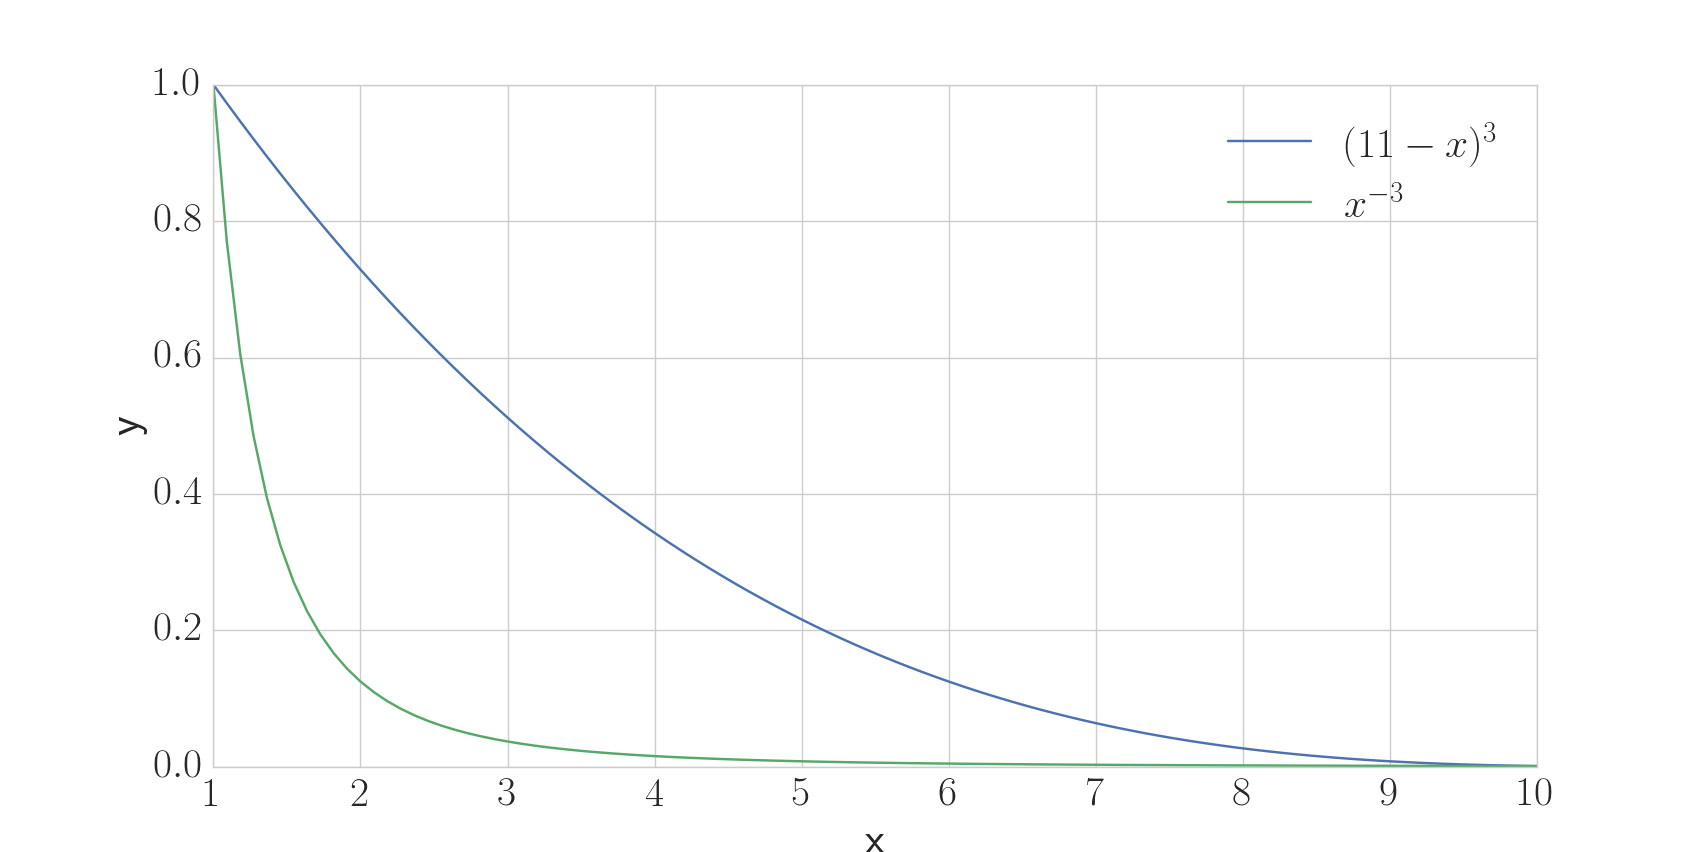
\includegraphics[width=13cm]{wrong_scaling.png}
  \caption{Comparision between the `hacked' negative exponent
    distribution and an actual negative power law
    distribution. Reflecting a positive power law about the y-axis
    does not result in a negative power law distribution.
    \label{fig:wrong_scaling}}
\end{figure}

Then I implemented the actual (tougher) concept of \textit{inverse
  transform sampling}, which takes random samples from a uniform
distribution between $[0,1)$ and converts them into samples from a
arbitrary PDF given that the CDF of this distribution is invertable.

The given PDF is:
\begin{equation}
  \label{eq:powerlaw}
  P(M|\theta) = cM^{\alpha} \quad \forall x \in [M_{min},M_{max}] \quad a < 0
\end{equation}

Some simple algebra gives the CDF of this distribution as:

\begin{equation}
  F(x) =  \left\{
  \begin{array}{ll}
    0 & x < M_{min} \\[0.5cm] \frac{x^{\alpha+1}-
      M_{min}^{\alpha+1}}{M_{max}^{\alpha+1}- M_{min}^{\alpha+1}} &
    M_{min}\leq x\leq M_{max}\\[0.5cm] 1 & x > M_{max} \\
  \end{array}
  \right.
\end{equation}

The inverse of this distribution is given in equation~\ref{eq:invcdf}
where $u$ is a uniform random variable.

\begin{equation}
  \label{eq:invcdf}
  H^{-1}(u) = \left[ M_{min}^{\alpha+1} + \left(M_{max}^{\alpha+1} -
    M_{min}^{\alpha+1}\right)u\right]^{\frac{1}{\alpha+1}}
\end{equation}

Implementing this to drawn the $N$ masses between $M_{min}=3 \,
M_{\odot}$, $M_{max}=15 \, M_{\odot}$ with $\alpha = -1.35$ gave the
right distribution (see figure~\ref{fig:powerlaw_masses}).

\begin{figure}[!h]
  \centering 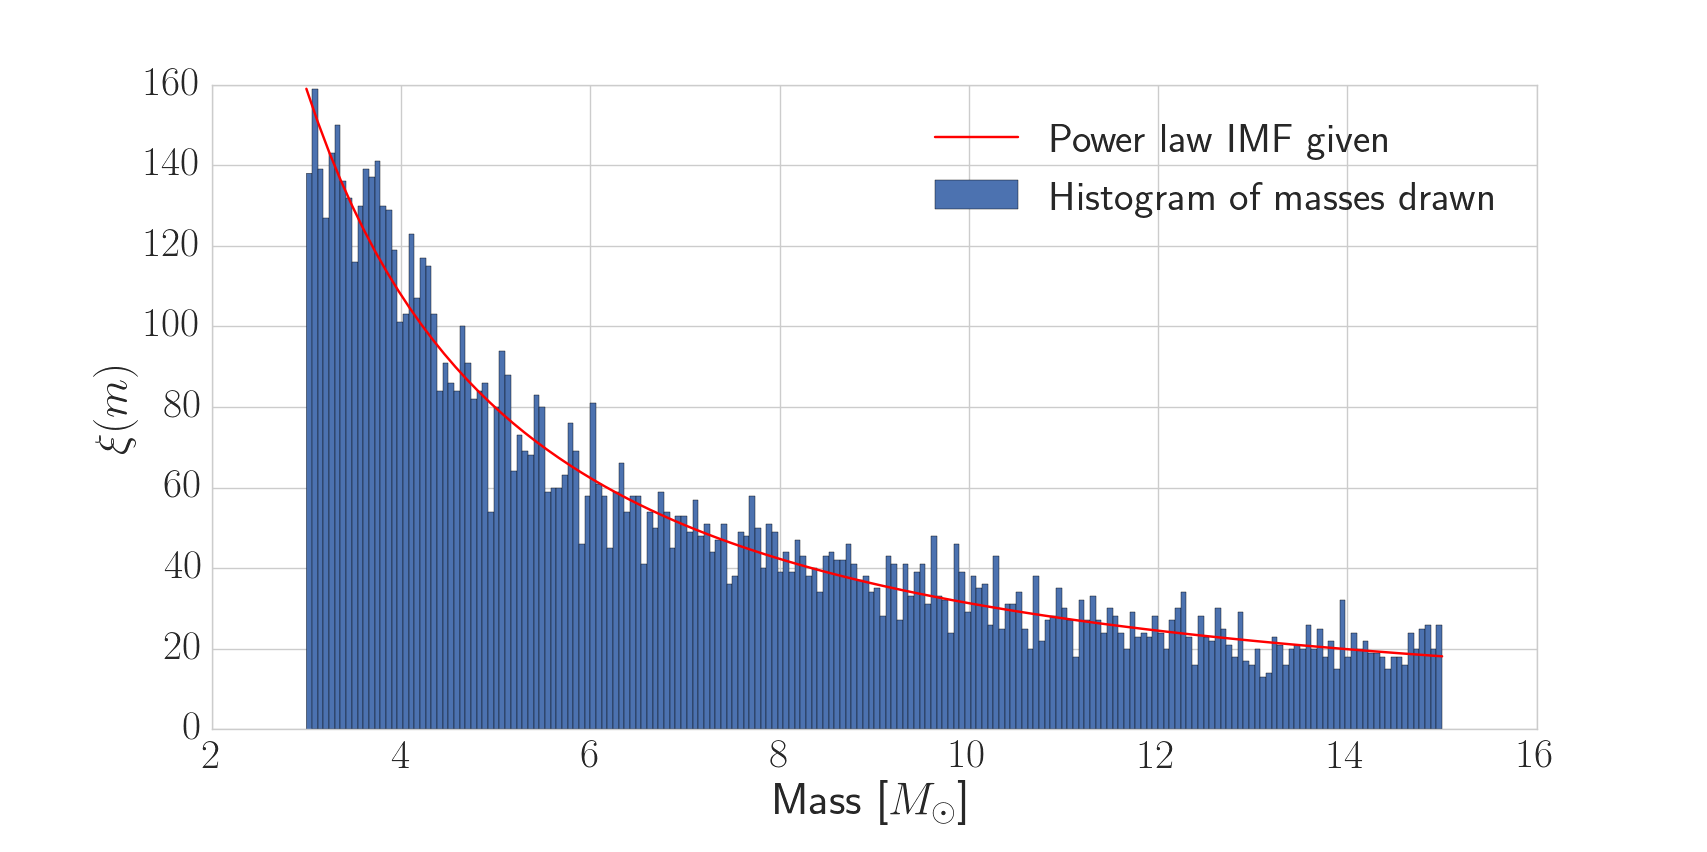
\includegraphics[width=13cm]{powerlaw_masses.png}
  \caption{Histogram of the masses drawn from the negative power law
    $cM^{-alpha}$ using inverse transform sampling, as compared to
    actual PDF. 
    \label{fig:powerlaw_masses}}
\end{figure}

(b) The trickiest part of this question was constructing the
log-likelihood function. Initially I tried computing the probability
of drawing the given masses, for the parameters $\theta =
(M_{max},\alpha)$ using the power law function (eq~\ref{eq:powerlaw})
but this did not work for some reason. The value of this estimator for
the `right' parameter set was somewhere inbetween the actual maximum
and minimum log-probability that \texttt{emcee} reported. Hence I
concluded that this might not be the right estimator and resort to
fitting the histogram in $\log-\log$ space which would just be a
straight line.


(c) This was the most troublesome, discouraging and teaching part of
the question.

The log-likelihood estimator I described above, yielded the right
value of the slope after correcting a few silly bugs but the reported
$M_{max}$ was very close to $M_{min}$. This took a few hours of
serious mulling over! When I tried to infer $M_{max}$ from the
intercept of the fit, I realised that the intercept was itself
wrong. Yet, I had normalised the CDF from which I drew my random
masses, which should have resulted in a normalised histogram-- did it?
No!

Even if masses were drawn from a normalized power law, the resulting
histogram of the masses was not normalized. Stranger still, the area
under the curve varied with the number of bins I was trying to
use. Only for very large number of bins was the area converging to 1,
but hold your horses before you make bins=N. Histograms of power law
distributions are not very indicative at the high mass end, intefering
with a good fit for $\alpha$. So the best resolution to this problem
was re-normalizing the histogram before fitting for $\alpha$ and
$M_{max}$.

It was a moment of euphoria to see the corner plot
(figure~\ref{fig:corner_1e3}) finally (finally!)  converge on
$M_{max}$ and $\alpha$ of nearly the right values. \texttt{corner}
seemed very confident with the estimate of the parameters but the
autocorrelation time reported by \texttt{emcee} was $\sim 25$
prompting me to manually compute the confidence interval. The 25th and
75th percentiles of $M_{max}$ and $\alpha$ are $(11.1,11.2)$ and
$(-1.29,-1.30)$ respectively. 

\begin{figure}[!h]
  \centering 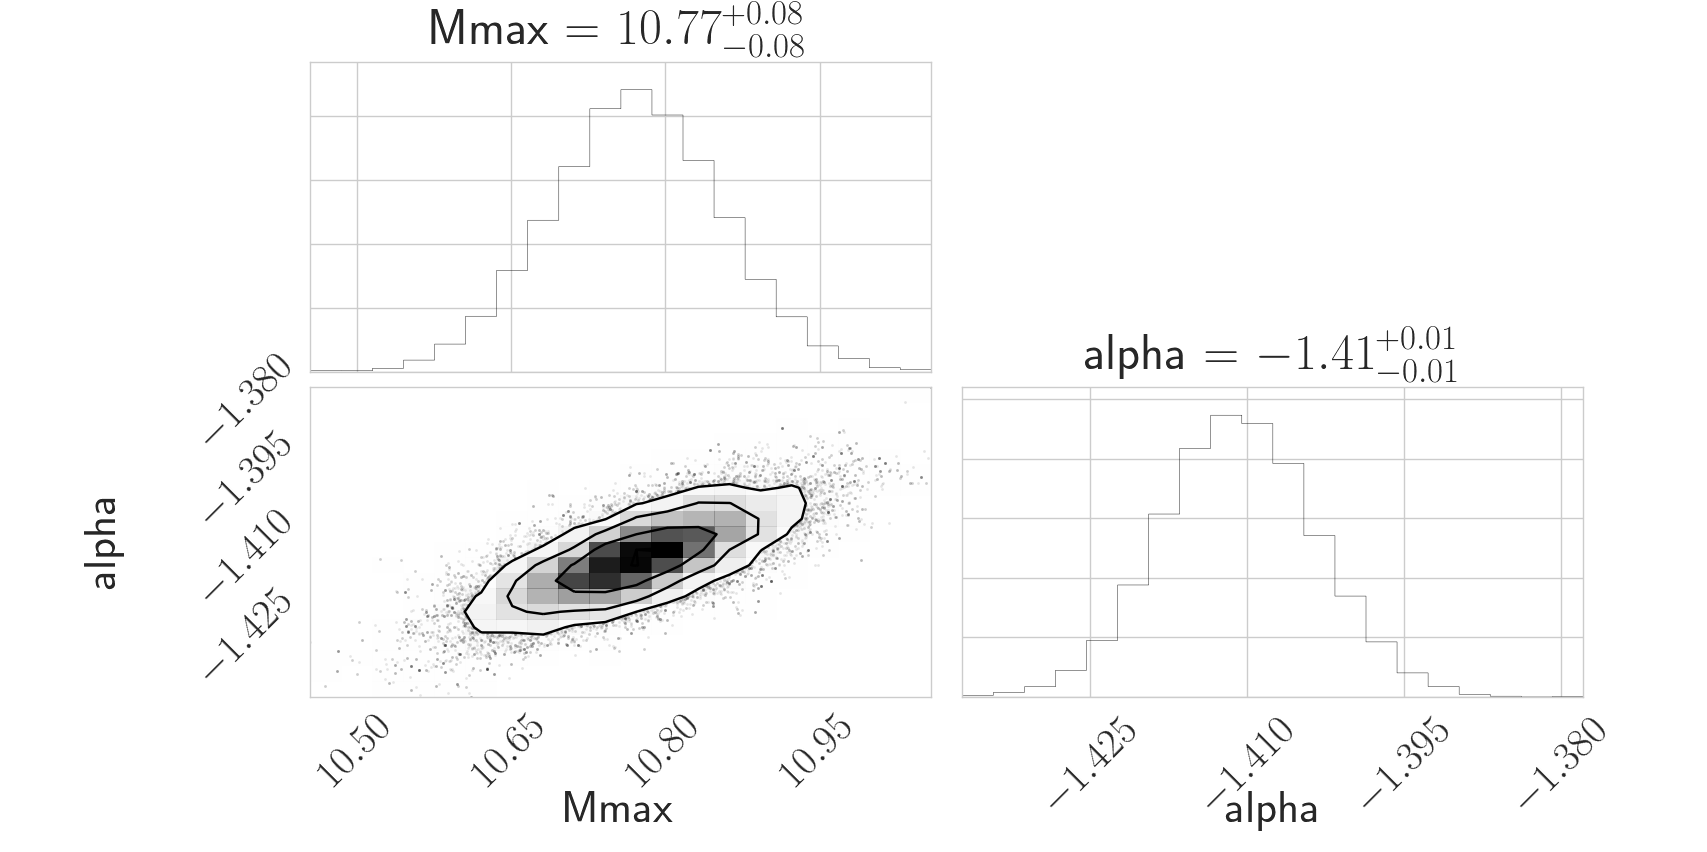
\includegraphics[width=13cm]{theta_1e3.png}
  \caption{The corner plot obtained after normalizing the area under
    the histogram with 10 bins and running \texttt{emcee} for 500
    steps using 300 walkers. The resulting values are close to the
    actual parameters of $\alpha = -1.35$ and $M_{max}=15$.
    \label{fig:corner_1e3}}
\end{figure}

After this experience it would have been worthwhile to check if the
original estimator I tried would work if the area under the power law
was normalized, but I did not have time to try this again.

(d) The plots obtained for different number of masses generated are
shown in figures~\ref{fig:corner_1e4}, ~\ref{fig:corner_1e2},
~\ref{fig:corner_1e1}. As expected, the errors increase as the number
of samples keeps getting smaller. The reported parameters for the N=10
case are so grossly erroneous that it makes me very skeptical of high
mass IMF estimates, since that is the region which is most hurt by
lack of data.

\begin{figure}[!h]
  \centering \includegraphics[width=13cm]{theta_q2.png}
  \caption{The corner plot obtained after normalizing the area under
    the histogram (bins=100) and running \texttt{emcee} for a 100
    steps with 200 walkers. The reported parameters for $N=10000$
    samples are very close to the actual values though the errors
    estimated might be incorrect.
    \label{fig:corner_1e4}}
\end{figure}

\begin{figure}[!h]
  \centering 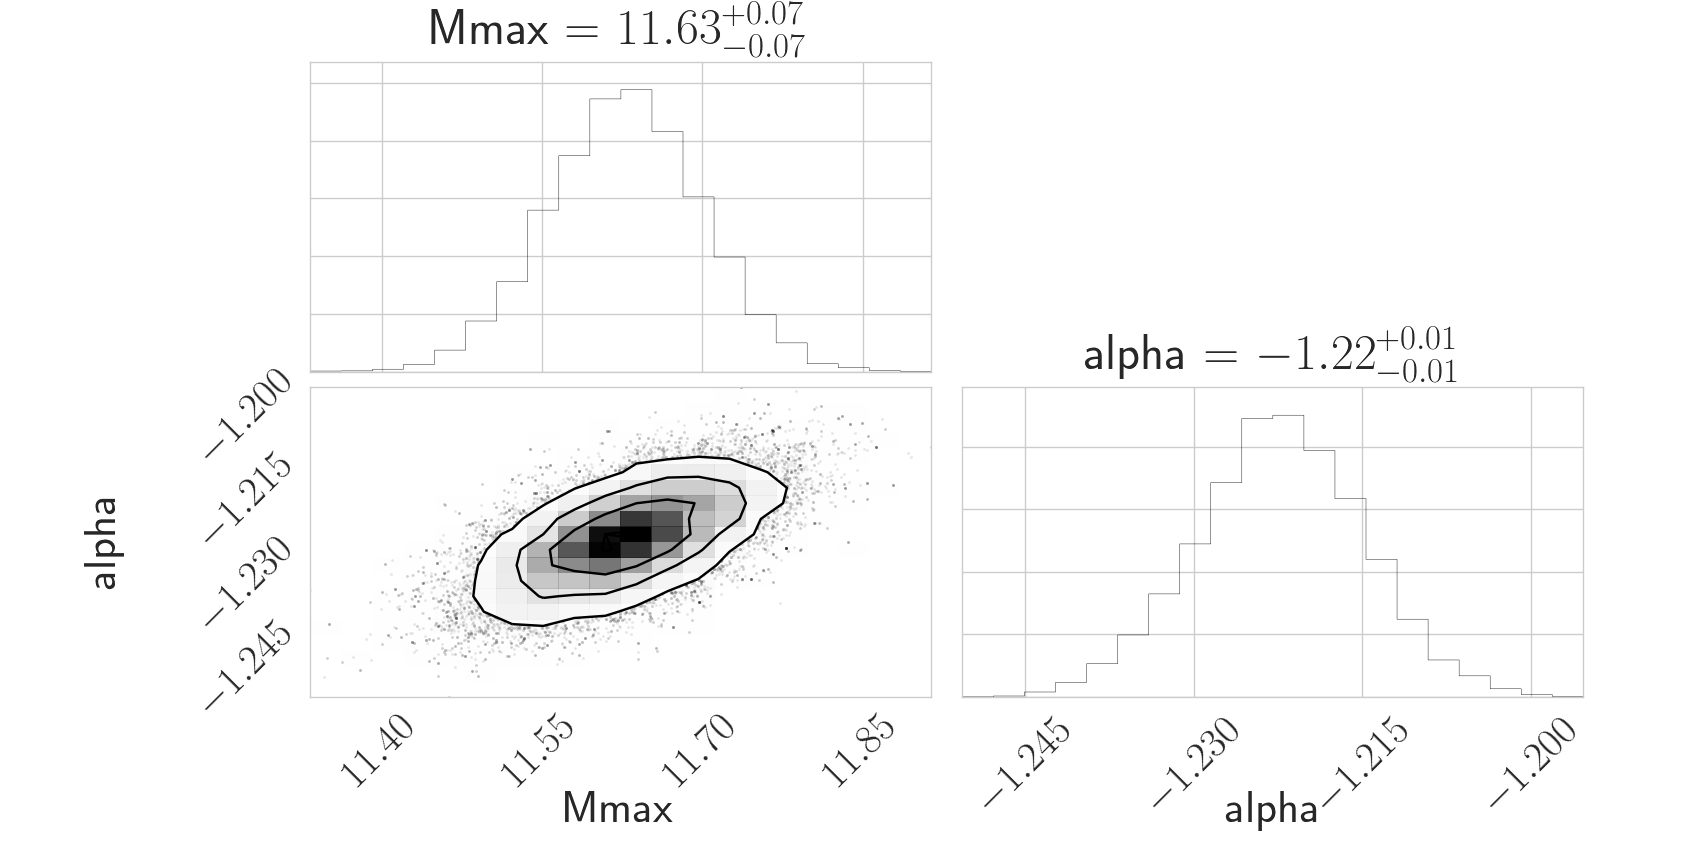
\includegraphics[width=13cm]{theta_1e2.png}
  \caption{Corner plot obtained by using $N=100$ samples with 10 bins,
    300 walkers and 500 steps. The reported slope is off by $0.2$ and
    the maximum mass by $5M_{\odot}$ making you wonder how scientists
    agree on the IMF even as much as they do!
    \label{fig:corner_1e2}}
\end{figure}

\begin{figure}[!h]
  \centering 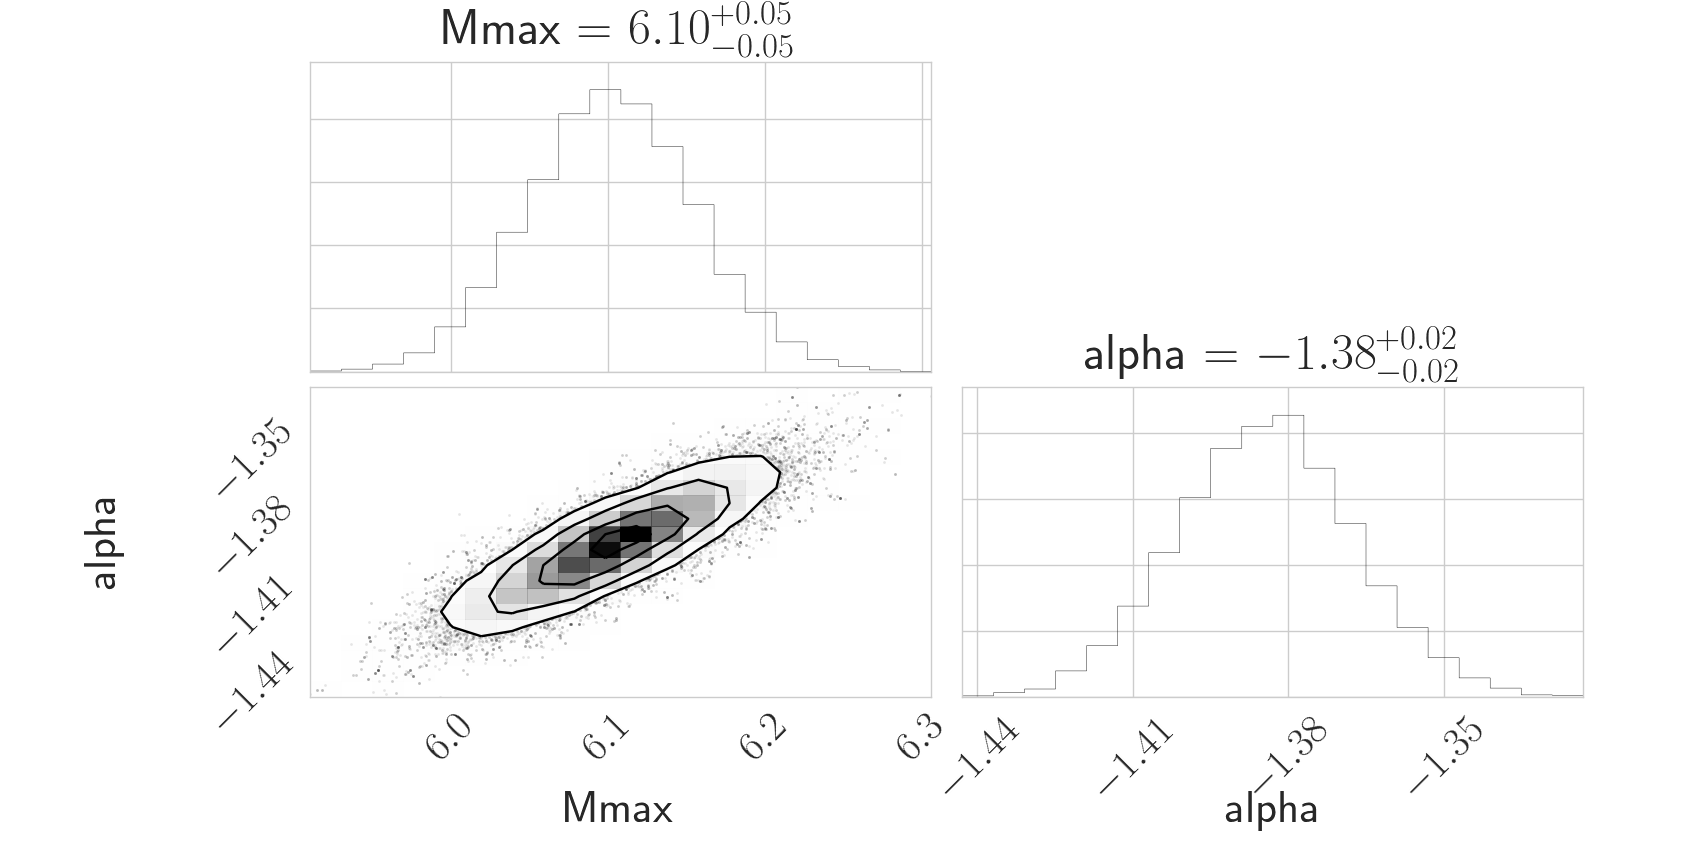
\includegraphics[width=13cm]{theta_1e1.png}
  \caption{Corner plot obtained for $N=10$ samples with 3 bins, 300
    walkers and 500 steps. The results are completely off as you would
    expect, but unfortunately you sometimes have to try to infer the
    power law slope with such less data. 
    \label{fig:corner_1e1}}
\end{figure}


\section{Problem 3}

In this problem, we will attempt to re-create Salpeter's original IMF
measurement.  \\

(a) Using the data for mass and number density in Table 2 and/or
Figure 2 in Salpeter (1955), fit a power-law using an optimizer or
least squares fitter (e.g., \texttt{scipy.optimize}).\\

(b) Same as part (a) only using your own inference code and
\texttt{emcee}.  Compare the two results: How close are they to one
another? How close are they to the value reported in Salpeter (1955)?
\\

\noindent \textbf{Solution:}

The code for this section is included in the repository under the very
intuitive name of \fbox{\texttt{q3.py}}

(a) This part was relatively straight forward. I used
\texttt{scipy.optimize.least\_squares} to find the optimum value for
the slope and intercept of the data in $\log-\log$ space. The slope
reported by scipy was \fbox{-1.40} as compared to Salpeter's slope of
$-1.35$.

(b) This part was very easy as compared to the last
question. \texttt{emcee} converged right away with a 100 walkers
making 1000 steps to give a slope of $-1.39$. As expected,
\texttt{scipy} and \texttt{emcee} are closer than Salpeter's estimate,
though his value comes very close when you remember that his work was
from 1955! Figure~\ref{fig:salp} compares the three results to each
other and the original data used.

\begin{figure}[!h]
  \centering 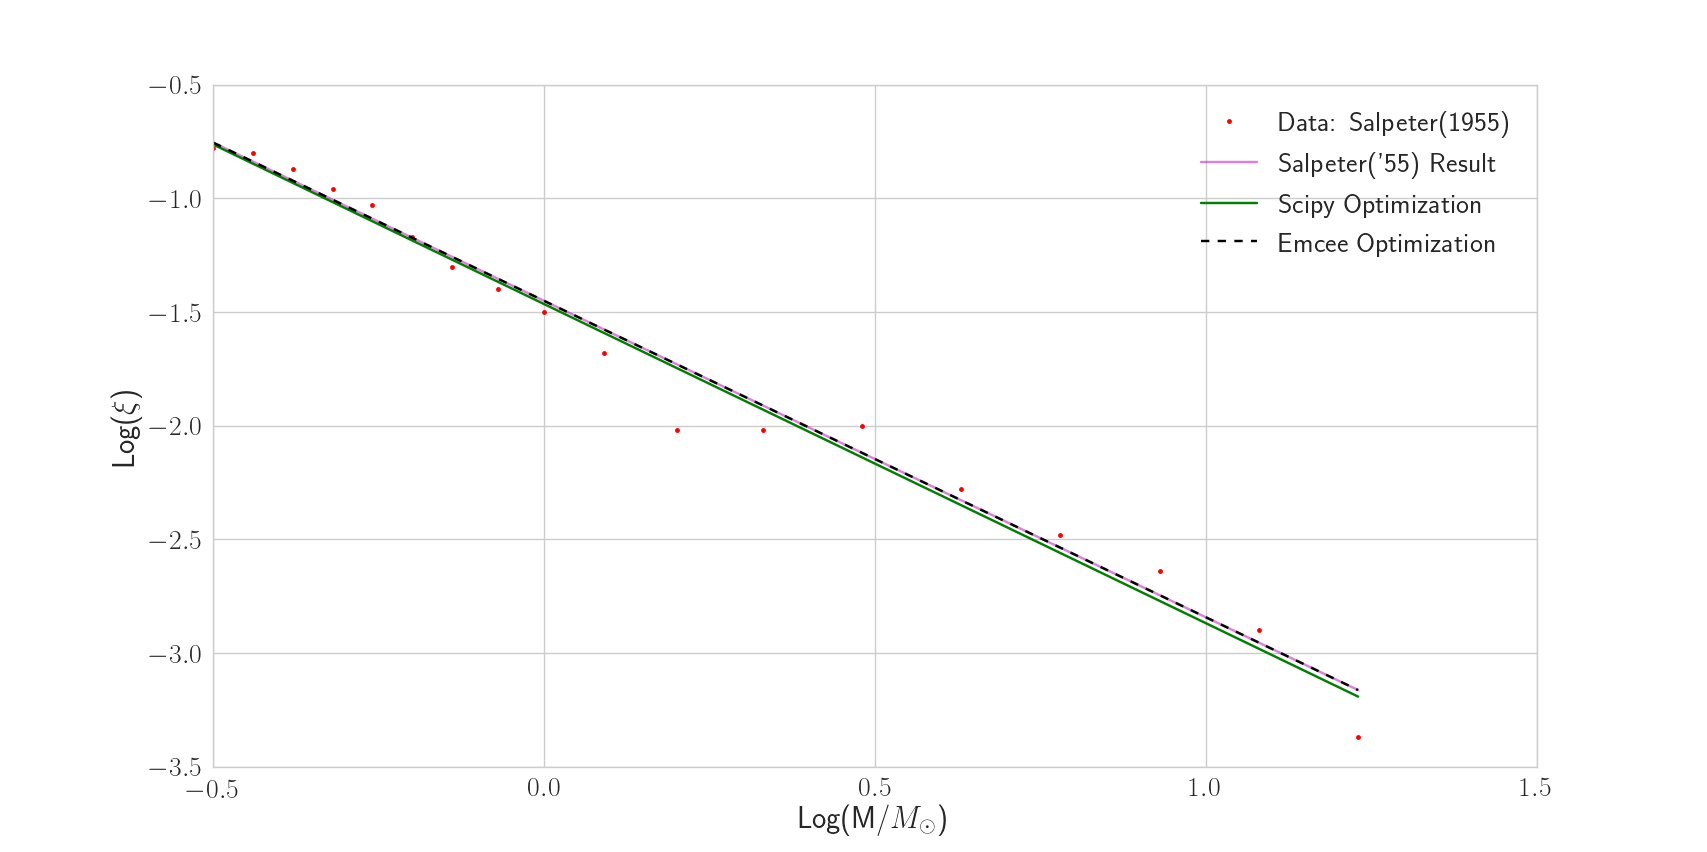
\includegraphics[width=13cm]{salpeter_imf.png}
  \caption{Comparision between the power law slope inferred by
    Salpeter in 1955, the modern day optimizing algorithm under the
    \texttt{scipy.optimize} package, and the MCMC algorithm
    implemented by \texttt{emcee}. The two 21st century algorithms
    agree better with each other than with Salpeter's calculations but
    the difference is almost negligible given the present day
    disagreements on the IMF.
    \label{fig:salp}}
\end{figure}

\section{Problem 4}

There are claims in the literature that the low-mass IMF slope may
systematically deviate from the Galactic value in low-mass dwarf
galaxies (e.g., Wyse et al. 2002; Geha et al. 2013).  However, these
measurements are made over a fairly limited mass range (usually $\sim
0.5- 0.8 \, M_{\odot}$) and done so assuming that a power-law is a
reasonable approximation for the low-mass IMF.

Suppose the true IMF for stars with $M<1 M_{\odot}$ in all galaxies is
actually a Chabrier IMF, i.e., a log-normal at low-masses.  Ignoring
corrections for stellar multiplicity, this IMF has the functional
form:

\begin{equation}
\xi(m)\Delta m = \frac{0.15}{m} \, {\rm exp}\frac{-(log(m) -
  log(0.08))^2}{(2\times0.69^2)}
\end{equation}

(a) Using the Chabrier IMF from above, generate a list of $N$=10,000
(perfectly known) stellar masses between 0.5 and 0.8 $M_{\odot}$.  \\

(b) Now, assuming a single-slope power-law IMF model (as done in the
literature), infer the value of the spectral index $\alpha$.  How does
this compare with the canonical Kroupa IMF found in the Milky Way?  \\

\noindent \textbf{Solution:}

\begin{figure}[!h]
  \centering 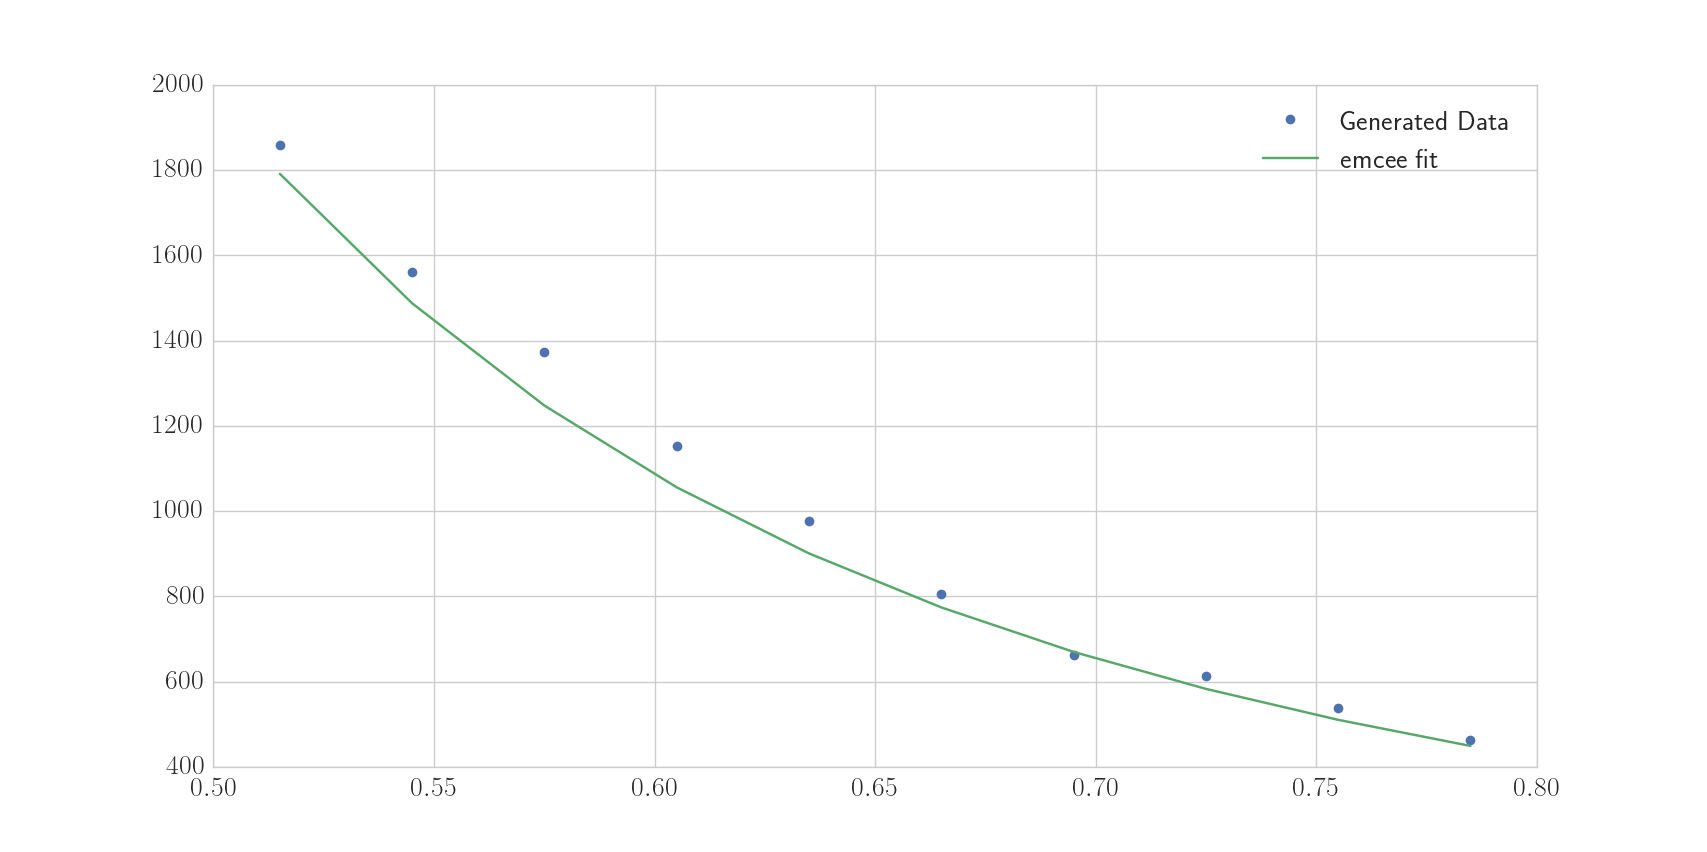
\includegraphics[width=13cm]{lognormal.png}
  \caption{
    \label{fig:lognorm}}
\end{figure}


\section{Problem 5}
Using python-FSPS: \\

(1) Generate the spectrum for a 10 Myr simple stellar population
(assume no dust, fixed metallicity, etc -- the only variable of
interest is age). Plot how the spectrum from $1500- 10000$\AA\ changes
for three different high-mass IMF ($>1\, M_{\odot}$) values:
$\alpha=0.8, 1.3, 1.8$, holding the lower portions of the IMF fixed.
\\

(2) Generate the spectrum of a 10 Gyr simple stellar population.  Plot
how the spectrum from $5000-20000$\AA\ changes for three different IMF
forms: Salpeter IMF, a Kroupa IMF, and the van Dokkum IMF.

\noindent \textbf{Solution}

(1)

\begin{figure}[!h]
  \centering 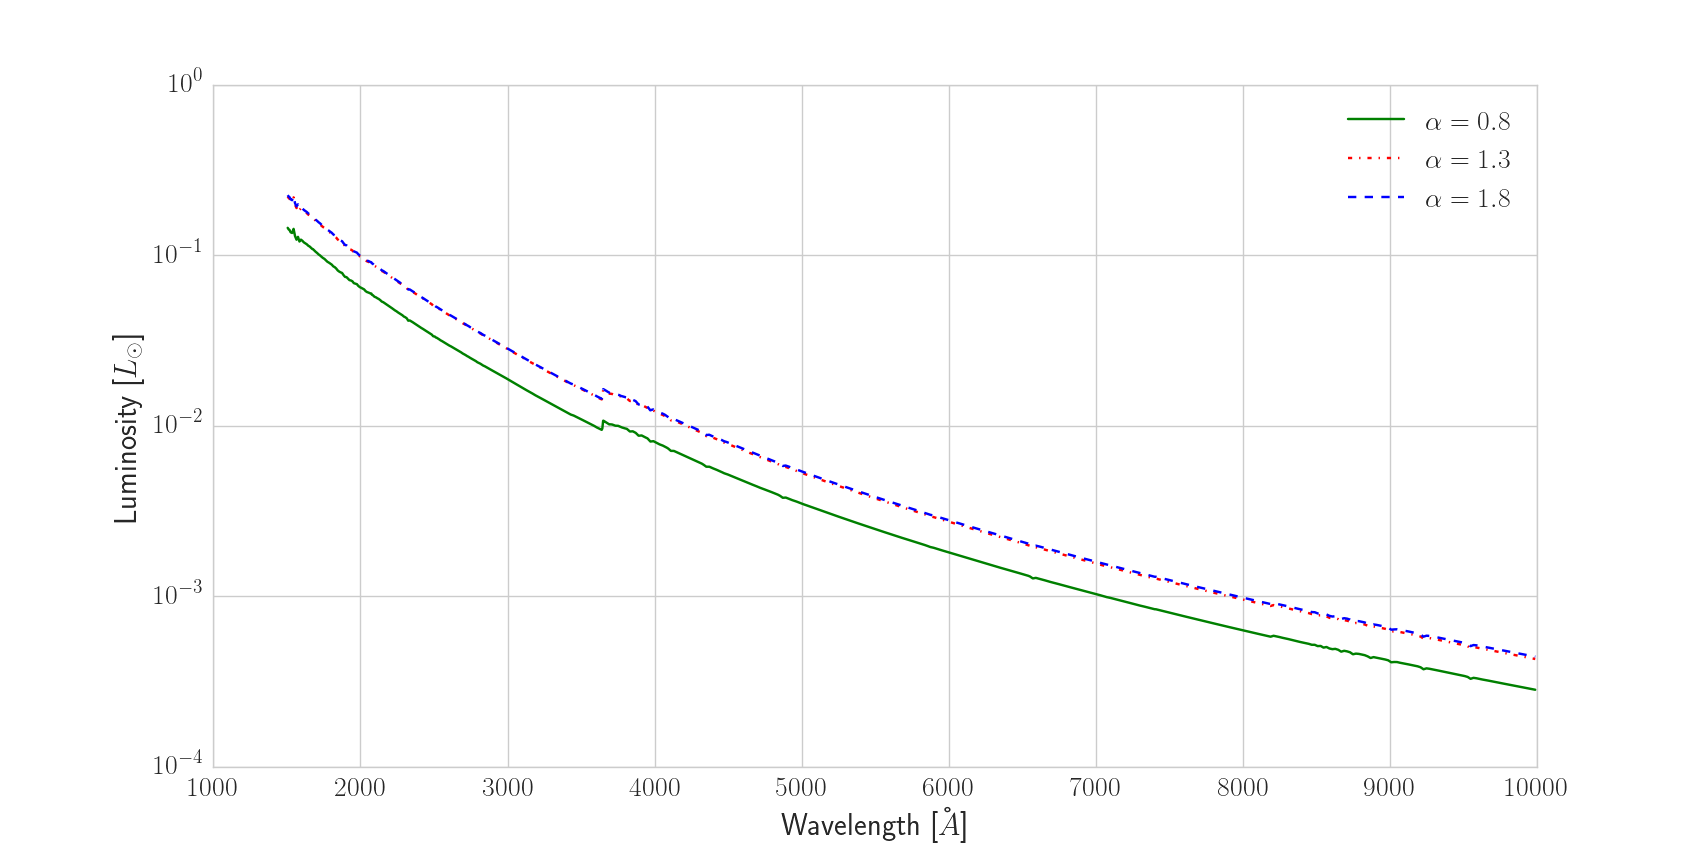
\includegraphics[width=13cm]{ssp_highmass_imf.png}
  \caption{
    \label{fig:ssphighmass}}
\end{figure}

\begin{figure}[!h]
  \centering 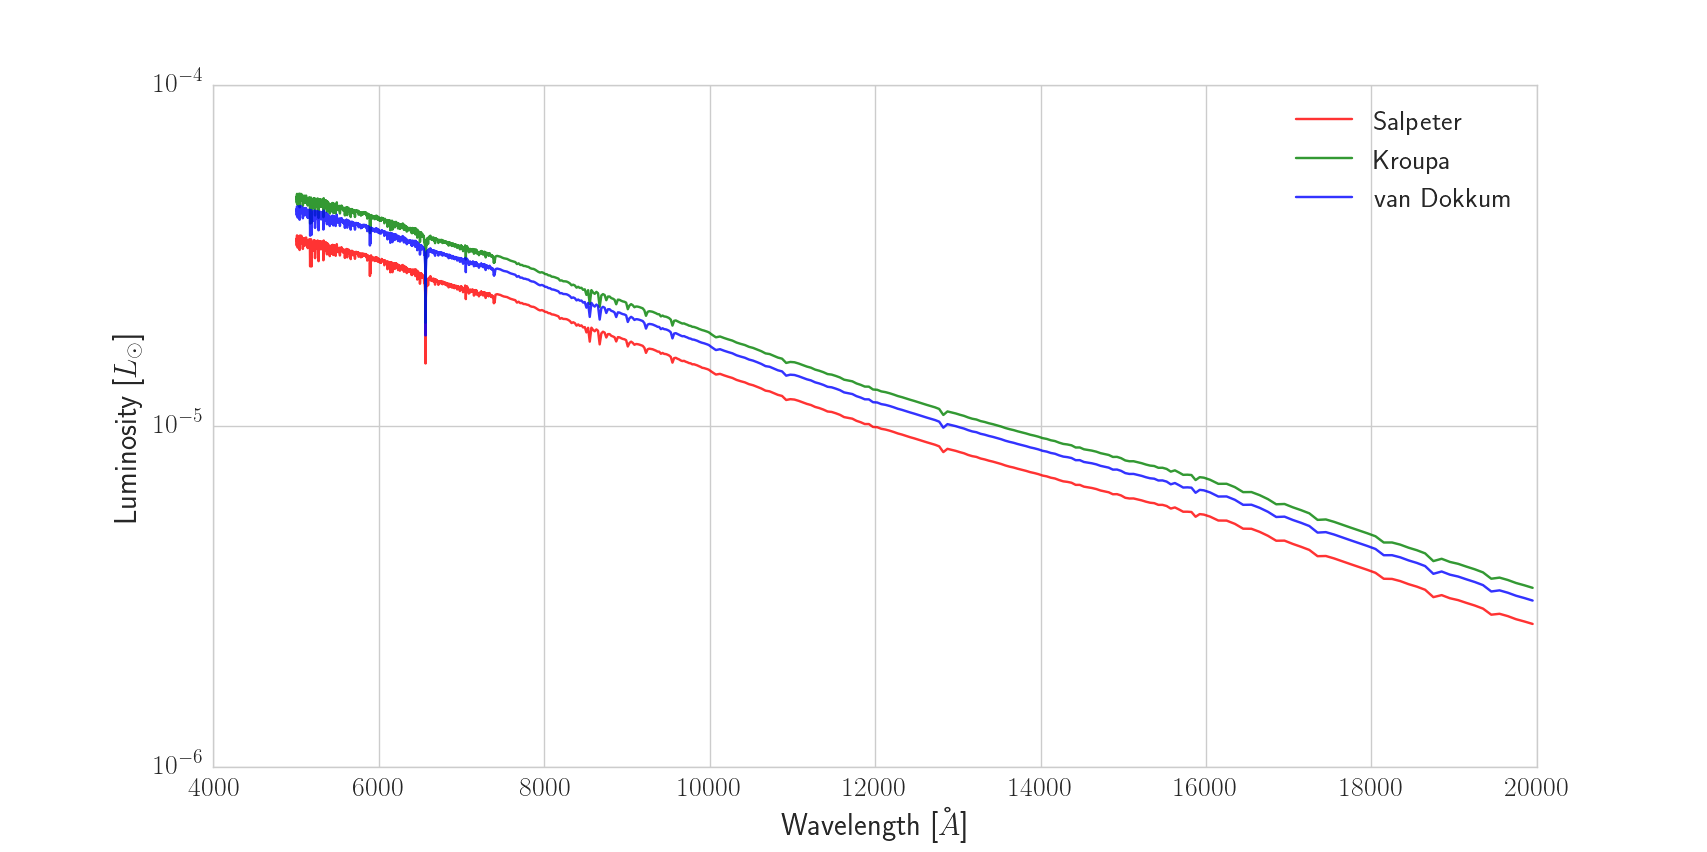
\includegraphics[width=13cm]{ssp_imfprofile.png}
  \caption{
    \label{fig:sspimf}}
\end{figure}

\end{document}
